\documentclass[omni.tex]{subfiles}

\begin{document}

\begin{figure}
{\begin{center}
    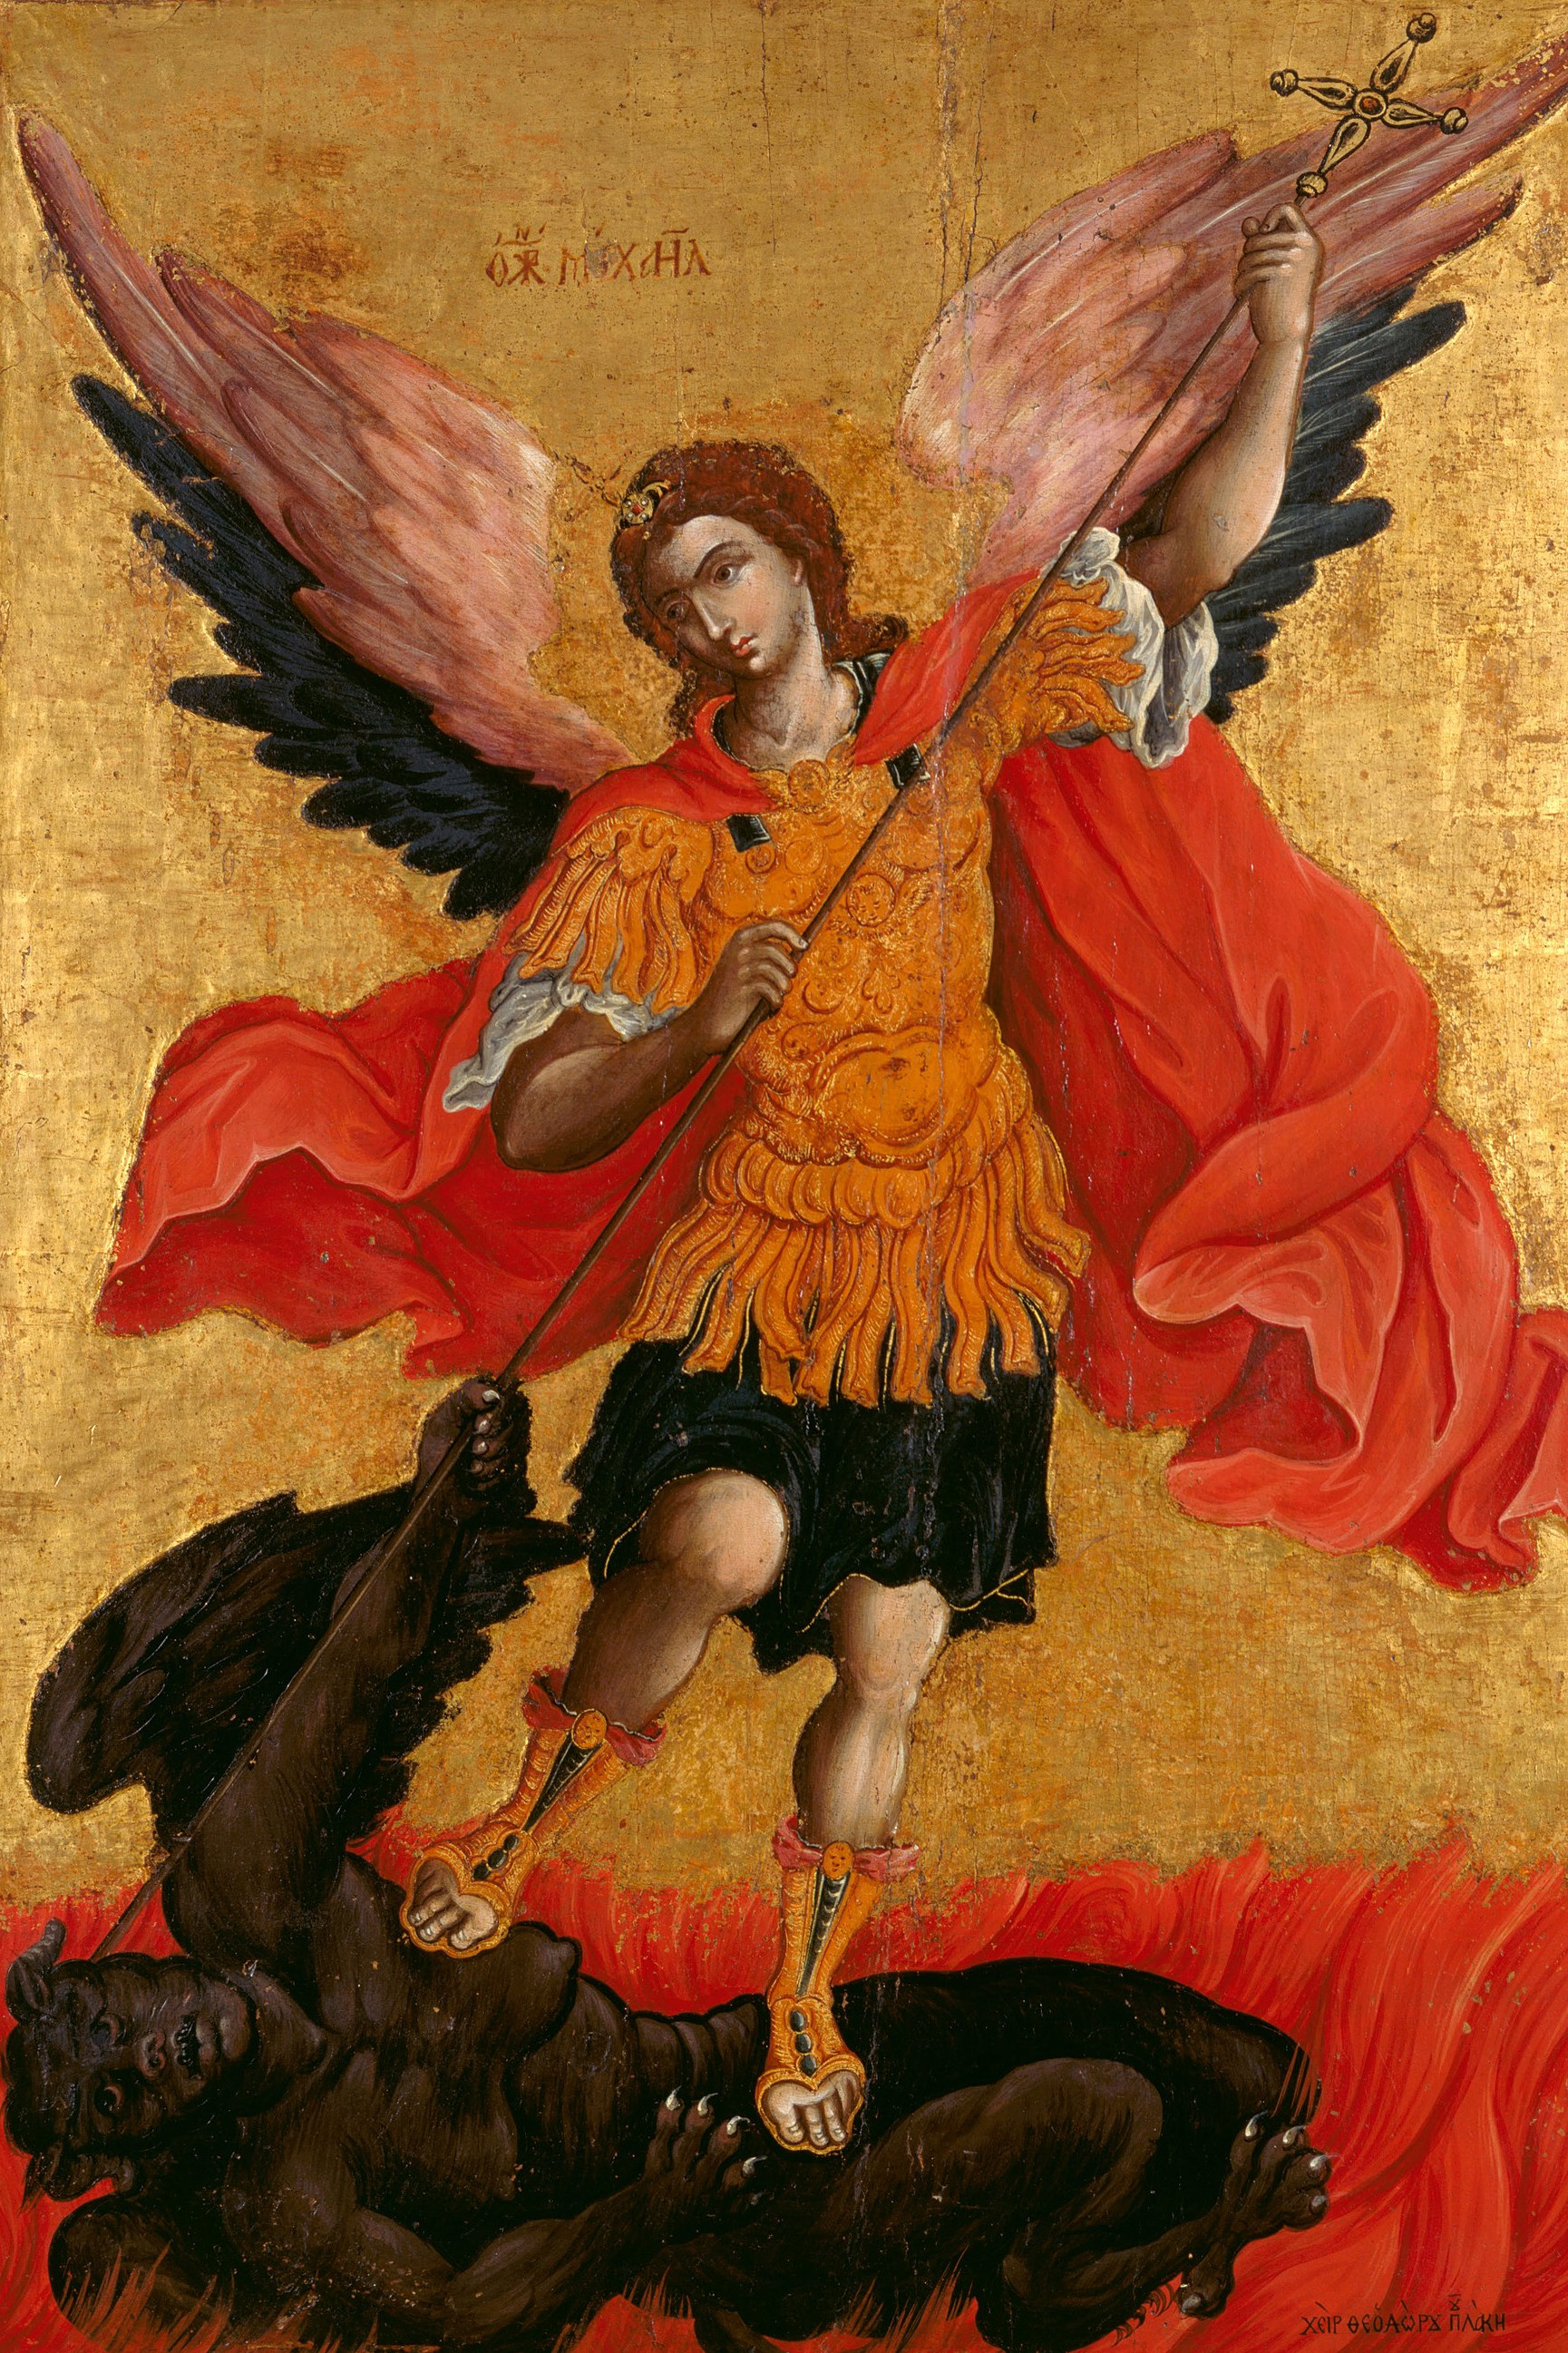
\includegraphics[width=2in]{sancte_michael}
\end{center}}
\end{figure}

\poemtitle{S\'ancte M\'ichael}
\settowidth{\versewidth}{Et ne nos ind\'ucas in tentati\'onem}

\begin{verse}[\versewidth]
\lettrine[lhang=1.0,nindent=0em]{S}{\'ancte M\'ichael} \\>
Arch\'angele, \\>
def\'ende nos in pro\'elio; \\
c\'ontra nequ\'itiam et ins\'idias \\
di\'aboli \'esto pr\ae s\'idium.
\end{verse}

\begin{verse}[\versewidth]
\'Imperet \'illi D\'eus, \\
s\'upplices deprec\'amur; tuque, \\
Pr\'inceps mil\'iti\ae\ c\ae l\'estis, \\
S\'atanam \\
ali\'osque sp\'iritus mal\'ignos, \\
qui ad perditi\'onem anim\'arum \\
pervag\'antur in m\'undo, \\
div\'ina virt\'ute, \\
in inf\'ernum detr\'ude. \\
\'Amen. \\[0\baselineskip]
\end{verse}
\attrib{IV}

\pagebreak
\end{document}
